


\section{Accretion \label{sect:accretion}}
{\color{blue}(10 pages)}
Accretion is the defining factor for young stars, it is through accretion that they build up mass, it is through accretion that they accumulate angular momentum, and it is probably through magnetic connection between disk and accretion column that at least some part of their angular momentum is lost. Once accretions stops, the mass, chemical composition, and angular momentum of a star only evolved very slowly through winds, on time scales similar to how main-sequence stars evolve.

Today it is widely accepted that the accretion in T Tauri stars is magnetically funneled. The accretion disk does not reach down to the stellar surface. Instead, it is truncated at a few stellar radii where the inner edge of the disk co-rotates with the central star. While magnetic fields of young stars can be complex, at large distances the field will be dominated by a dipole component. Magnetic field lines couple to the inner disk and the disk material, ionized by the UV and X-ray radiation from the star, is forced to follow the field lines. As it falls in, gravity accelerates the matter to free-fall velocity until it hits the surface where a strong shock develops \cite{shu_94}. 

We first look at the accretion stream and the locations of the footpoints. Then, we describe the picture of simple-1D accretion shock  before we extend this to more detailed observations and models.

\subsection{The accretion stream and its foot points}
\label{sect:accretionsrteam}
The accretion stream is initially cool; it heats up as mass accelerates and comes close to the star. The most prominent tracers are the strong and complex hydrogen emission lines. In particular H$\alpha$ is usually optically thick, often shows red-shifted absorption components compatible with free-fall velocity \cite[e.g.][]{2000AJ....119.1881A}, and varies over time scales of hours \cite{dupree_2012}. Many emission lines do not vary with the stellar rotation period, indicating that it is the inner disk, not the anchor point on the stellar surface, that controls the geometry of accretion \cite{2021A&A...649A..68S}.

Zeeman-Doppler imaging can reveal the structure of the magnetic field and, using certain assumptions, those fields can be extrapolated out to the inner disk edge. There seems to be an evolution of magnetic field strength and geometry, where the strength of the dipole component, which dominates the field at large radii and is thus most important for coupling to the accretion disk and carrying the accretion funnel, decreases with the depth of the convective envelope \cite{2012ApJ...755...97G,2019A&A...622A..72V}. On the stellar surface itself, doppler imaging can locate the position of the accretion funnels which are often found near the pole as in BP Tau \cite{2008MNRAS.386.1234D} or V2129 Oph \cite{2011A&A...530A...1A}, but sometimes at lower latitudes as in V2247 Oph \cite{2010MNRAS.402.1426D}. Simulations can reproduce the analytical model of accretion foot points near the pole in the dipolar field, but they also point to more complex geometries when disk, stellar rotation, and stellar magnetic field are not aligned, see Fig.~\ref{fig:romanova} for an example.

\begin{figure}[t]
\centering
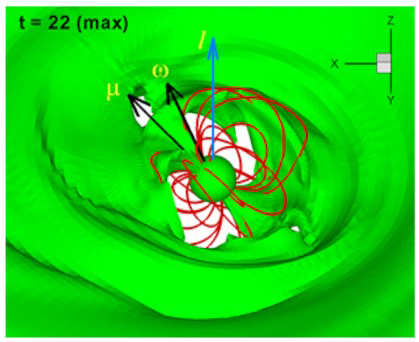
\includegraphics[width=5cm]{figs/Romanova2021fig8-panel.png}
\caption{Simulation of accretion on an inclined dipole. Mass flows towards the magnetic pole \cite{2021MNRAS.506..372R} \textcolor{blue}{need to ask for permission} \label{fig:romanova}}
\end{figure}

How do we know if the X-ray emission, which we associate with the shock, actually originates at the same location as the optical lines used for Doppler imaging? In one case, TW Hya, the signal is strong enough to determine the line shift of the soft X-ray lines to $38.3 \pm 5.1$~km/s \cite{2017A&A...607A..14A}. Since this is much less then the free-fall velocity, we much see the shock close perpendicular to the line-of-sight. TW~Hya is observed close to pole-on, so the accretion shocks must the located in the equatorial region.




\subsection{X-ray signatures of the accretion shock}
\label{sect:accretionobs}
{\color{blue}Moritz, Christian

Kastner & Brickhouse spectra, other spectra?, Argiroffi redshift? yes, Brickhouse 2012 variability,  naturepaper solar!, argiroffi V2129, V4046}


% Moritz list of citations to be put in the correct location later
AA Tau?

MHD modelin coal abs 2014ApJ...795L..34B 

2011A&A...526A.104C curran



The X-ray emission from cool stars on the main-sequence (MS) is caused by coronal activity. Young stars rotate faster and thus have more magnetic activity and thus also stronger coronal X-rays than older MS stars such as our Sun. That is why accretion signatures are hard to find in broad-band X-ray spectra, in particular for stars embedded in a molecular cloud. To the contrary, surveys even show reduced X-ray flux correlated with accretion \cite{2005ApJS..160..401P}. However, this does not contradict the idea that accretion shocks generate soft X-rays as models show that the shock would contribute only below 1~keV \cite{1999AstL...25..430L}.

Additional diagnostics are provided by high-resolution grating spectroscopy from Chandra or XMM-Newton \cite{Kastner_2002}. Most importantly, the density of the emitting plasma can be determined from line ratios in the O~{\sc vii} and Ne~{\sc ix} triplets, which can be resolved into three lines with XMM-Newton or Chandra grating spectroscopy: A resonance line ($r$), an intercombination line ($i$), and a forbidden line ($f$). In collisionally excited plasma, the $f$ line is typically stronger than the $i$ line, but collisions in high-density plasma or strong UV fields (relevant in A or B stars, but not in the lower-mass classical T Tauri stars) can excite an electron from the upper level of the $f$ line to the upper level of the $i$ line. A low $f/i$ ratio is thus a sign of high densities in the emission region, which leads to the idea that this X-ray emission originates behind the shock front of an accretion shock.

\begin{figure}[t]
\centering
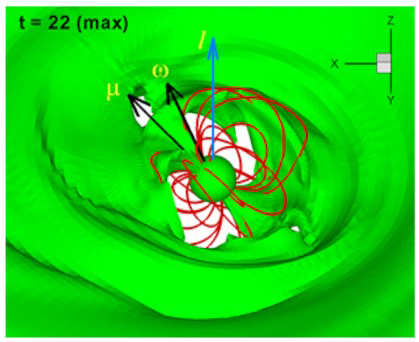
\includegraphics[width=5cm]{figs/Romanova2021fig8-panel.png}
\caption{Text here. Modified from:  \cite{2013ApJ...771...70G} \label{fig:softexcess}}
\end{figure}

Ref.~\cite{Guenther_2007} compared XMM-Newton data from TW~Hya to updated models that explicitly predicted these density-sensitive line ratios and could explain the available data of TW~Hya at the time. In this case, about two thirds of the total X-ray flux must be due to the shock, with the remaining emission coming from a stellar corona. However, deeper observations, again for TW~Hya \cite{Brickhouse_2010}, 


\subsection{Physics of accretion in 1D}
\label{sect:accretionphysics}
{\color{blue}(free-fall, accretion shock, plasma temperature, X-ray emission, etc.) [Moritz, Sabina]
Accretion sketch Hartmann et al. 2016 - we might use our own picture, too.

}

Accretion happens when mass from the circumstellar disk is transferred onto the stellar surface. In the basic model of magnetically funneled accretion, the stellar high-energy radiation ionizes the inner edge of the disk. When the stellar magnetic field connects to the inner edge of the disk, matter can flow along the field lines and impact onto the star, where a strong shock forms. The accretion column is relatively cool, but in the shock that gas is heated up to X-ray emitting temperatures. Depending on the exact location of the shock, those X-rays may or may not be visible, but the shock certainly heats the surrounding photosphere, which causes bright UV emission and an optical veiling (a strong continuum that makes phtotospheric emission lines appear weaker than in a non-accretion star.)

As the star and the disk rotate, and the magnetic field and the disk structure evolves, the accretion geometry and the accretion rate can change on time scales as short as minutes or as long as centuries; accretion can also switch off temporarily or permanently, as the star looses its disk. Despite that, many basic aspects of the accretion physics can be described in a 1D model where all mass motion happens parallel to the magnetic field. In the next few sub-sections we review some of the basic physics of accretion columns and accretion shocks. While modern models go far beyond such a simple prescription, the foundation of all accretion shock models still is to convert the graviational energy in the disk to kinetic energy of the infalling gas, which in turn gets turned into heat and radiation in the accretion shock.

\subsubsection{Free-fall velocity}
The free fall velocity $v_{\textnormal{free}}$ of material coming from an inner disk radius of $R_\mathrm{in}$ onto a star with mass $M_*$ and radius $R_*$ is
\begin{equation} 
v_{\textnormal{free}} = \sqrt{{2GM_*} \left(\frac{1}{R_*} - \frac{1}{R_\mathrm{in}}\right)} \approx 620 \sqrt{\frac{M_*}{M_\odot}}\sqrt{\frac{R_\odot}{R_*}} \frac{\textnormal{km}}{\textnormal{s}}\ \label{eqn:freefall} 
\end{equation}
where $G$ is the gravitational constant. The inner radius is typically a few stellar radii and thus $v_\textnormal{ff}$ is very close to infall from infinity.


\subsection{Calculation of shock front}
All turbulent fluxes are neglected and we only treat stationary shocks. In the shock front, ions and electrons are heated differently, but they remain strongly coupled and reach the same temperatures with in a few mean-free path lengths - a region so thin that it is justified to treat them as a single fluid. 

Somewhere along the accretion column, a shock forms when the forward ram pressure becomes comparable to the pressure of the underlying material. The shock front itself is very thin, only of the order of a few mean free paths \cite{raizerzeldovich}. Therefore it can be treated as a mathematical discontinuity described by the Rankine-Hugoniot jump-conditions \cite[][chap.~7, \S~15]{raizerzeldovich}; in the shock the super-sonic infall velocity is converted mostly into thermal energy. To simplify the numerical treatment we assume the direction of flow parallel to the magnetic field, so the Lorentz force does not influence the dynamics. Marking the state in front of the shock front by the index 0, that behind the shock by index 1, the Rankine-Hugoniot conditions become
\begin{eqnarray}
\rho_0 v_0 &=& \rho_1 v_1 \label{RH1}\\
P_0+\rho_0 v_0^2 &=& P_1+\rho_1 v_1^2 \label{RH2}\\
\frac{5 P_0}{2\rho_0}+\frac{v_0^2}{2}&=&\frac{5 P_1}{2\rho_1}+\frac{v_1^2}{2} \ ,\label{RH3}
\end{eqnarray}
where $v$ is the velocity, $\rho$ the total mass density of the gas and $P$ its pressure. 

From the jump conditions, the shocks will heat gas to a temperature
$$
kT \simeq \frac{3}{16}\mu m_p v^{2} \approx 0.3\,{\rm keV}\left(\frac{v}{500\,{\rm km/s}}\right)^{2},
\label{eqn:Tshock}
$$
where $\mu$ is the dimensionless atomic weight.

\subsubsection{Structure of the post-shock region}

In the following section we compute how the originally different kinetic temperatures of ions and electrons as well as the ionisation temperature
equilibrate and calculate the emitted X-ray spectrum.

\paragraph{Momentum balance}\label{hydrodyn}

In the post-shock region the gas emits radiation and cools down, so the energy of the gas is no longer conserved.  However, the particle number flux $j$ of ions (and atoms) 
\begin{equation}j=nv\label{j_n}\end{equation}
is conserved, where $n$ is the ion/atom number density; the electron number density is denoted by $n_{\mathrm{e}}$. The total momentum flux $j_p$ is conserved, since we ignore the momentum loss by radiation; it consists of the ion and the electron momentum as follows:
\begin{eqnarray}  
j_p&=&\mu m_{\mathrm{H}} n v^2+P \nonumber \\
   &=&\mu m_{\mathrm{H}} n v^2+nkT \label{j_p}
\end{eqnarray}
with $P$ is the thermodynamic pressure and $T$ the temperature; $m_{\mathrm{H}}$ denotes the mass of a hydrogen atom.

\paragraph{Energy balance}
\label{sect:energybalance}

Let us next consider the energy balance in the post-shock region. In general,  
\begin{equation} \label{tsminuspdvisdu} T d\Sigma -P dV=dU \end{equation}
where $\Sigma$ denotes the entropy and $U$ the internal energy of the plasma. The quantity $T d\Sigma=dQ$ denotes the heat flux through the boundaries of the system; one important component of the is the energy loss $Q_{col}$ through collisions that excite higher electronic states, which will than decay through radiation. 

Assuming that the shock location is stationary, we get $\frac{d}{dt}=\frac{\partial}{\partial t}+\frac{\partial z}{\partial t}\frac{\partial}{\partial z}=v\frac{\partial}{\partial z}$ depending on the location $z$, measured from the shock front inwards; differentiation with respect to $z$ will be indicated by $'$.
The internal energy $U$ is in this case the thermal energy $U=\frac{3}{2}kT$, the pressure $P$ can be rewritten using the equation of state. The specific volume $V$ is the inverse of the number density $V=\frac{1}{n}$. 
It is convenient to write the electron number density as \mbox{$n_{\mathrm{e}}=x_e n$,} with $x_e$ denoting the number of electrons per heavy particle.
\begin{equation}
\label{energyelec}
v\left(\frac{3}{2}x_e k T_{\mathrm{e}}\right)'+v x_e n k T_{\mathrm{e}} \left(\frac{1}{n}\right)'=-Q_{col} x_e n,
\end{equation} 

We now have $n$, $v$, and $T$ as variables and three hydrodynamic equations (\ref{j_n}, \ref{j_p}, and \ref{energyelec}), so the structure of the post-shock region can be calculated.


\subsection{Models}

\label{sect:accretionmodels}
{\color{blue}(historic evolution of models and aspects addressed by models) [Moritz, (Sabina)]

Accretion column models Lamzin 2004, Robinson & Espaillat?; C IV lines (Lamzin 2003?); accretion rates



Radiative transfer (Colombo et al. )


}

\begin{figure}
    \centering
    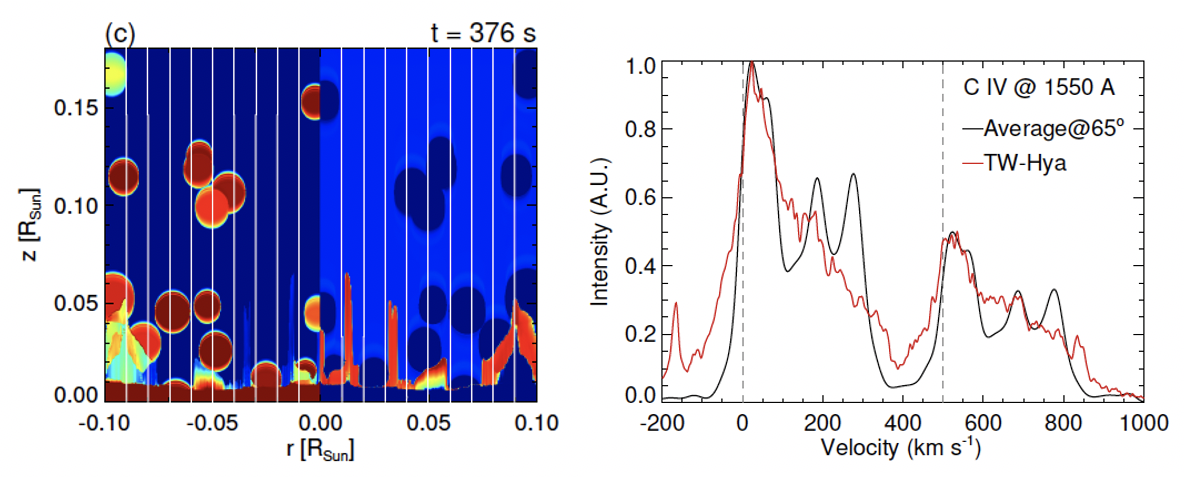
\includegraphics[width=11cm]{figs/colombo2016.png}
    \caption{A combination of Fig. 3 and Fig. 6 from Colombo et al. 2016. Interesting for the fragmented structure of the accretion stream which reproduces the CIV profiles (X-rays and other observations). Need for permission. I would select one of the figures, Colombo 2016 or Colombo 2019b.}
    \label{fig:colombo2016}
\end{figure}

\begin{figure}
    \centering
    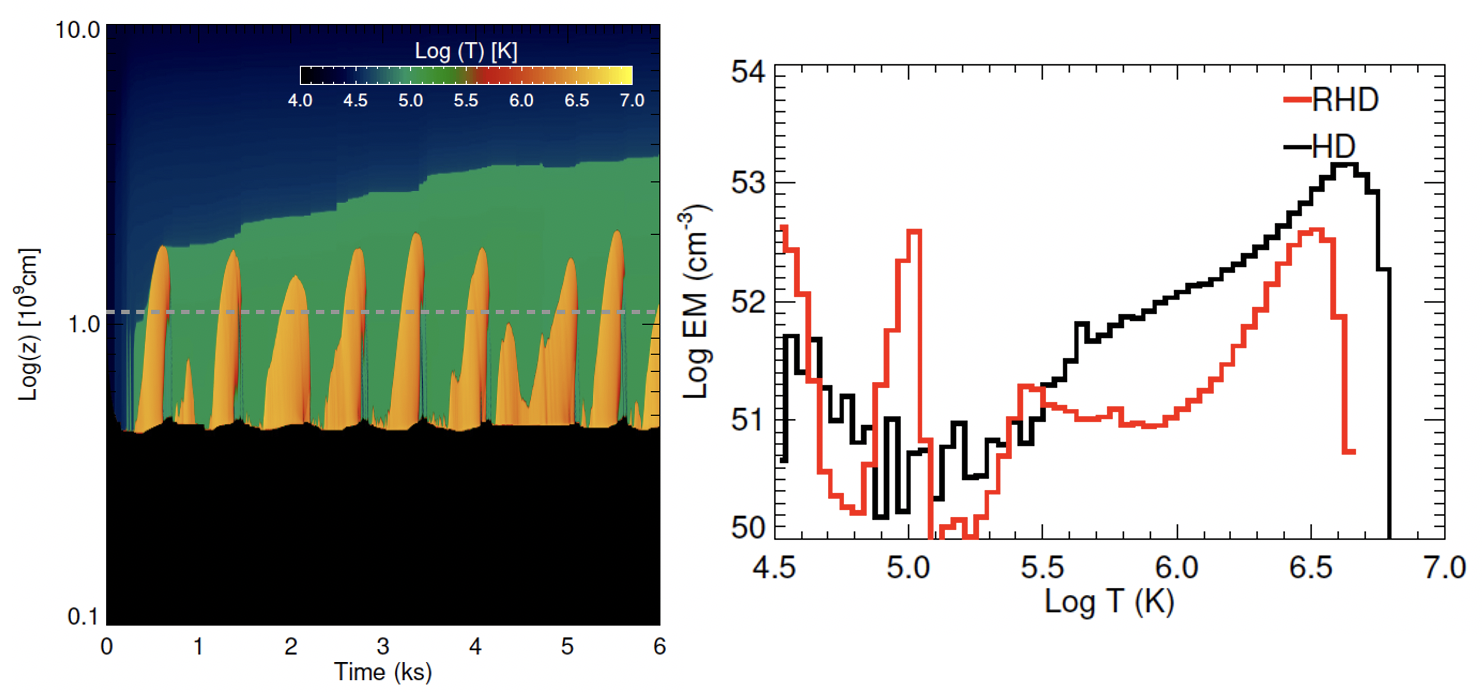
\includegraphics[width=11cm]{figs/colombo2019b.png}
    \caption{A combination of Fig. 3 and Fig. 5 from Colombo et al. 2019b. As far as I know the only non-LTE simulation of the accretion region. Need from permission. I would select one of the figures, Colombo 2016 or Colombo 2019b.}
    \label{fig:colombo2016}
\end{figure}

Early simulations follow the 1D prescription given above, which was sufficient to explain the high-energy data at the time. They show that the accretion shock produces plasma matching the observed X-ray temperatures \citep{lamzin_1998} and that the total energy in the accretion stream can be determined from fitting UV and optical spectra to determine the mass accretion rate \citep{calvet_1998}.

Using high-resolution grating spectroscopy from Chandra \citet{Kastner_2002} introduced additional diagnostics. Most importantly, the density of the emitting plasma can be determined from line ratios in the O~{\sc vii} and Ne~{\sc ix} triplets, which can be resolved into three lines with XMM-Newton or Chandra grating spectroscopy: A resonance line ($r$), an intercombination line ($i$), and a forbidden line ($f$). In collisionally excited plasma, the $f$ line is typically stronger than the $i$ line, but collisions in high-densities plasma or strong UV fields (relevant in A or B stars, but not in the lower-mass classical T Tauri stars) can excite an electron from the upper level of the $f$ line to the upper level of the $i$ line. A low $f/i$ ratio is thus a sign of high densities in the emission region, which leads to the idea that this X-ray emission originates behind the shock front of an accretion shock.

\citet{Guenther_2007} compared XMM-Newton data from TW~Hya to updated models that explicitly predicted these density-sensitive line ratios and could explain the available data of TW~Hya at the time. In this case, about two thirds of the total X-ray flux must be due to the shock, with the remaining emission coming from a stellar corona. However, deeper observations, again for TW~Hya \cite{Brickhouse_2010}, 

camer, birckouse, accretion stream, orlando

Similarly, improved models including LTE radiation transfer now show that the heated photosphere does not radiate as a simple black body in the optical and infrared \cite{Dodin_2012,Dodin_2013}, but that is also produces lines, which selectively fill in some photospheric absorption lines, possibly biasing accretion rate measurements based on optical veiling.

Shoud out to global models pf the accretion stream (romanova, etc.)

\subsection{The multi-D structure of the accretion shock}

Most observations of the structure of the accretion shock on young stars are spatially unresolved; only Doppler-imaging can at least reveal the location on the surface where the accretion shock happen. Yet, it would be very valuable to learn about the detailed 3D geometry and the time evolution of accretion shocks to interpret the unresolved data. For example, it is unclear if the accretion shocks forms deeply in the photosphere where it is hidden from view or higher up in the accretion funnel. One approach to address this problem is to perform experiments in the laboratory using a set-up where magnetic fields, densities, temperatures, and other hydrodynamical parameters are chosen to scale to the stellar case. Such work finds that plasma is ejected laterally from the accretion shock and forms a shell around the infalling stream \cite{2017SciA....3E0982R} . This hot shell provides an additional absorber that reduces the shock emission that is directly observable. Recently, new laboratory experiments tested accretion streams not perpendicular to the impacted surface as it might happen for accretion stream along complex magnetic field structures. They find the resulting plasma flows to be highly asymmetric and see a large amount of plasma escaping laterally from the accretion flow \cite{2020A&A...642A..38B}.  

Another approach is to look for analogous situations in our Sun, where spatially resolved data in the UV and EUV, even if not in X-rays, is available with long time coverage and high cadence. One particular event happened on June, 7$^{th}$, 2011, when parts of an erupting filament fell back into the Sun \cite{2013Sci...341..251R,2013A&A...559A.127O}. The infall speed of up to 450~km/s was comparable to free-fall accretion onto T Tauri stars, but the accretion rate was obviously much lower. Similar to the laboratory experiments, the initial infall triggered upflows, but here they shocked with later fragments causing UV emission.

Both, laboratory experiments and the solar analogy, point to a significantly more complex picture than the simple 1D accretion shock outlined in section~\ref{sect:accretionphysics}. Simulations of the accretion shock 


might explain low m rates... nh in TW hya , MHD simulations here...
